\documentclass[11pt,a4paper]{article}
\usepackage[utf8]{inputenc}
\usepackage[T1]{fontenc}
\usepackage[margin=0.9in]{geometry}
\usepackage{amsmath,amssymb,amsfonts}
\usepackage{booktabs}
\usepackage{graphicx}
\usepackage{hyperref}
\usepackage{microtype}
\usepackage{siunitx}
\usepackage{tikz}
\usepackage{xcolor}
\usepackage{enumitem}
\usepackage{fancyhdr}
\usepackage{tcolorbox}
\usepackage{array}
\usepackage{float}
\usepackage{caption}

\pagestyle{fancy}
\fancyhf{}
\setlength{\headheight}{14pt}
\fancyhead[L]{\footnotesize \textbf{NCSSM Connect} $\cdot$ Honors Aerospace Engineering}
\fancyhead[R]{\footnotesize \textbf{WindTunnel lab} $\cdot$ Simulation Results}
\fancyfoot[C]{\footnotesize \thepage}

\hypersetup{
    colorlinks=true,
    linkcolor=blue!70!black,
    citecolor=blue!70!black,
    urlcolor=blue!70!black
}

\tcbset{
    colback=gray!6!white,
    colframe=blue!70!black,
    fonttitle=\bfseries,
    boxrule=1pt,
    arc=4pt,
    left=8pt, right=8pt, top=5pt, bottom=5pt
}

\captionsetup{font=small,labelfont=bf}
\emergencystretch=1.5em

\title{\vspace{-1.8cm}\textbf{\huge Collaborative Wind Tunnel Flight Investigation}\\[0.15cm]
\textbf{\Large Complete Simulation Results \& Multi-Variable Stall Analysis}\\[0.1cm]
\normalsize Empirical Calibration of $\alpha_{\text{stall}} = K \cdot (t/c)^a \cdot (1+m)^b \cdot Re^c$ via GPU-Accelerated 2D LBM-LES \\
\vspace{0.1cm}
\small \textbf{Platform:} NCSSM \textit{WindTunnel lab} (D2Q9 BGK-Smagorinsky Lattice Boltzmann Solver)}
\author{\textbf{Aerospace Research Consortium Telemetry \& Analysis Report (\texttt{SimResults})} \\
Honors Aerospace Engineering $\cdot$ NCSSM Connect Program $\cdot$ NCSSM}
\date{November 2026}

\begin{document}
\maketitle
\vspace{-0.65cm}

\begin{tcolorbox}[title=Executive Summary of Consortium Findings, colframe=blue!65!black]
\small
Using the GPU-accelerated 2D D2Q9 Lattice Boltzmann Method with Smagorinsky Large-Eddy Simulation (\textbf{WindTunnel lab}), all 18 angle-of-attack ($\alpha$) sweeps specified across \textbf{Team 1 ($\Pi_1 = t/c$)}, \textbf{Team 2 ($\Pi_2 = m$)}, and \textbf{Team 3 ($\Pi_3 = Re$)} were executed under the standardized \textbf{5.0-second cycle-averaged Data Acquisition (DAQ)} protocol (200 display frames $= 4{,}000$ LBM steps per angle after a 4,000-step settling transient, totaling $>2.6 \times 10^6$ lattice updates).
\begin{itemize}[leftmargin=*, itemsep=1pt, topsep=2pt]
    \item \textbf{Empirical Power-Law Exponents:} Ordinary Least Squares (OLS) log-log regressions across the three orthogonal parameter sweeps yield:
    \begin{equation}
        a = 0.335 \pm 0.054 \ (R^2 = 0.951), \quad
        b = 1.612 \pm 0.322 \ (R^2 = 0.893), \quad
        c = 0.091 \pm 0.021 \ (R^2 = 0.869).
    \end{equation}
    \item \textbf{Unified General Stall Law:} Combining the three orthogonal scalings with baseline calibration on \texttt{NACA 0012} ($Re = 1000, \alpha_{\text{stall},0} = 16.0^\circ \Rightarrow K = 17.045^\circ$) yields the predictive design law:
    \begin{equation}
        \boxed{\alpha_{\text{stall}}\!\left(m,\, \frac{t}{c},\, Re\right) = 17.045^\circ \cdot \left(\frac{t}{c}\right)^{0.335} \cdot \left(1 + m\right)^{1.612} \cdot Re^{0.091}}
    \end{equation}
    \item \textbf{Out-of-Sample Coupled Validation:} Tested on off-axis multi-parameter airfoils never used in fitting, the unified law predicts $\alpha_{\text{pred}} = 13.45^\circ$ vs.\ $\alpha_{\text{meas}} = 13.50^\circ$ on \textbf{\texttt{NACA 4406}} (\textbf{$0.34\%$ error}) and $\alpha_{\text{pred}} = 19.57^\circ$ vs.\ $\alpha_{\text{meas}} = 19.00^\circ$ on \textbf{\texttt{NACA 4418}} (\textbf{$3.02\%$ error}).
\end{itemize}
\end{tcolorbox}

\vspace{-0.15cm}
{\footnotesize\tableofcontents}
\vspace{0.3cm}
\hrule
\vspace{0.3cm}

% =============================================================================
\section{Computational Methodology \& Aerodynamic Flow Regimes}
% =============================================================================

\subsection{D2Q9 Lattice Boltzmann Solver \& Cycle-Averaged DAQ Protocol}
All simulations were conducted on a two-dimensional Cartesian lattice of dimensions $N_x \times N_y = 800 \times 300$ lattice units ($\text{lu}$) using the nine-velocity $\text{D2Q9}$ lattice model with single-relaxation-time Bhatnagar--Gross--Krook (BGK) collision and a dynamic Smagorinsky subgrid-scale turbulence model ($C_s = 0.15$). The airfoil chord length is fixed at $c = 0.16 N_x = 128\text{ lu}$ with the leading edge positioned at $x_{\text{LE}} = 0.22 N_x = 176\text{ lu}$ and pivoted about the aerodynamic quarter-chord $(x_{c/4}, y_{c/4}) = (208, 150)\text{ lu}$. A uniform freestream inflow velocity $u_{\text{in}} = 0.08\text{ lu/step}$ ($\text{Ma} = u_{\text{in}}/c_s \approx 0.139 \ll 0.3$, ensuring incompressible flow) is prescribed at $x = 0$, zero-gradient convective outflow at $x = N_x - 1$, free-slip specular walls at $y \in \{0, N_y - 1\}$, and half-way bounce-back on solid airfoil nodes.

For any prescribed Reynolds number $Re = u_{\text{in}} c / \nu$, the kinematic lattice viscosity and bare relaxation time are determined by:
\begin{equation}
    \nu = \frac{u_{\text{in}}\,c}{Re}, \qquad \tau_0 = \frac{1}{2} + \frac{3\,u_{\text{in}}\,c}{Re}, \qquad \tau_{\text{eff}}(\mathbf{x}, t) = \frac{\tau_0 + \sqrt{\tau_0^2 + 18\sqrt{2}\,C_s^2\,\|\boldsymbol{\Pi}^{\text{neq}}(\mathbf{x}, t)\|_F/\rho}}{2}.
\end{equation}
Instantaneous fluid forces $\mathbf{F} = (F_x, F_y)$ acting on the airfoil perimeter are evaluated at every lattice step via the Galilean-invariant \textbf{Momentum Exchange Method (MEM)}:
\begin{equation}
    \mathbf{F} = \sum_{\mathbf{x}_b \in \partial\Omega_{\text{solid}}} \sum_{i=1}^{8} 2\,\mathbf{c}_i\,f_i^{\text{in}}(\mathbf{x}_b, t), \qquad C_D = \frac{F_x}{\frac{1}{2}\rho_0 u_{\text{in}}^2 c}, \qquad C_L = \frac{F_y}{\frac{1}{2}\rho_0 u_{\text{in}}^2 c},
\end{equation}
where dynamic pressure per unit span is $q_\infty c = \frac{1}{2}\rho_0 u_{\text{in}}^2 c = 0.5 \times 1.0 \times (0.08)^2 \times 128 = 0.4096$.

To eliminate post-stall vortex-shedding bias, each angle of attack $\alpha$ was allowed to settle for $200\text{ frames}$ ($4{,}000\text{ steps} \approx 2.5$ convective flow-through times), followed by a standardized \textbf{5.0-second DAQ recording window} ($N = 200\text{ frames} = 4{,}000\text{ steps}$). Within each 200-frame buffer, a 3-point moving-average filter identifies local maxima ($k_{\max}$) and minima ($k_{\min}$) separated by at least 6 frames. Whenever $\ge 2$ peaks and $\ge 1$ trough are detected (unsteady periodic vortex shedding), time integration is truncated to an \textbf{exact integer number of vortex-shedding cycles} $[k_{\text{first}}, k_{\text{last}}]$, recording $\overline{C_L}$, $C_{L,\min}$, $C_{L,\max}$, $\sigma_{C_L}$, $\overline{C_D}$, $\sigma_{C_D}$, and $\overline{L/D} = \overline{C_L}/\overline{C_D}$.

\subsection{Two-Stage Stall Topology in 2D Low-\texorpdfstring{$Re$}{Re} Flows: Primary Attached Stall vs.\ Secondary Vortex Lift}
A defining physical feature of two-dimensional laminar-to-transitional airfoils at $Re \in [300, 5000]$ is the presence of \textbf{two distinct lift peaks} during an angle-of-attack sweep (illustrated in Figure~\ref{fig:flow_fields}):
\begin{enumerate}[leftmargin=*, itemsep=2pt]
    \item \textbf{Primary Attached-Flow Stall Peak ($\alpha_{\text{stall}}, C_{L,\text{stall}}$):} Occurs in the stall zone $\alpha \in [12.0^\circ, 19.0^\circ]$ when the laminar boundary layer detaches from the upper surface under the adverse pressure gradient $\partial p/\partial x > 0$. This point marks the \textit{first confirmed local lift maximum} followed by a lift drop ($\Delta C_L \ge 0.035$) and the collapse of aerodynamic efficiency $(L/D)$. In accordance with classical aerodynamic definition and the automated stall detector in \texttt{WindTunnel lab}, $\alpha_{\text{stall}}$ and $C_{L,\text{stall}}$ define the primary boundary-layer stall point used for all scaling laws.
    \item \textbf{Secondary Leading-Edge Vortex (LEV) Peak ($\alpha_{\text{LEV}}, C_{L,\max}$):} At deeper post-stall incidences ($\alpha \in [18.5^\circ, 21.5^\circ]$), periodic roll-up of the detached leading-edge shear layer generates intense Leading-Edge Vortices (LEVs) that convect across the chord before shedding into a von K\'arm\'an vortex street. In 2D (where spanwise vortex stretching is absent), these coherent LEVs induce a secondary suction wave that temporarily drives cycle-averaged lift to a higher global peak $C_{L,\max}$ at the cost of massive form drag ($C_D > 0.35$) and violent structural buffeting ($\Delta C_L > 0.4$). Both $C_{L,\text{stall}}$ (primary stall) and $C_{L,\max}$ (global LEV peak) are reported in the Master Telemetry Table.
\end{enumerate}

\begin{figure}[!htbp]
    \centering
    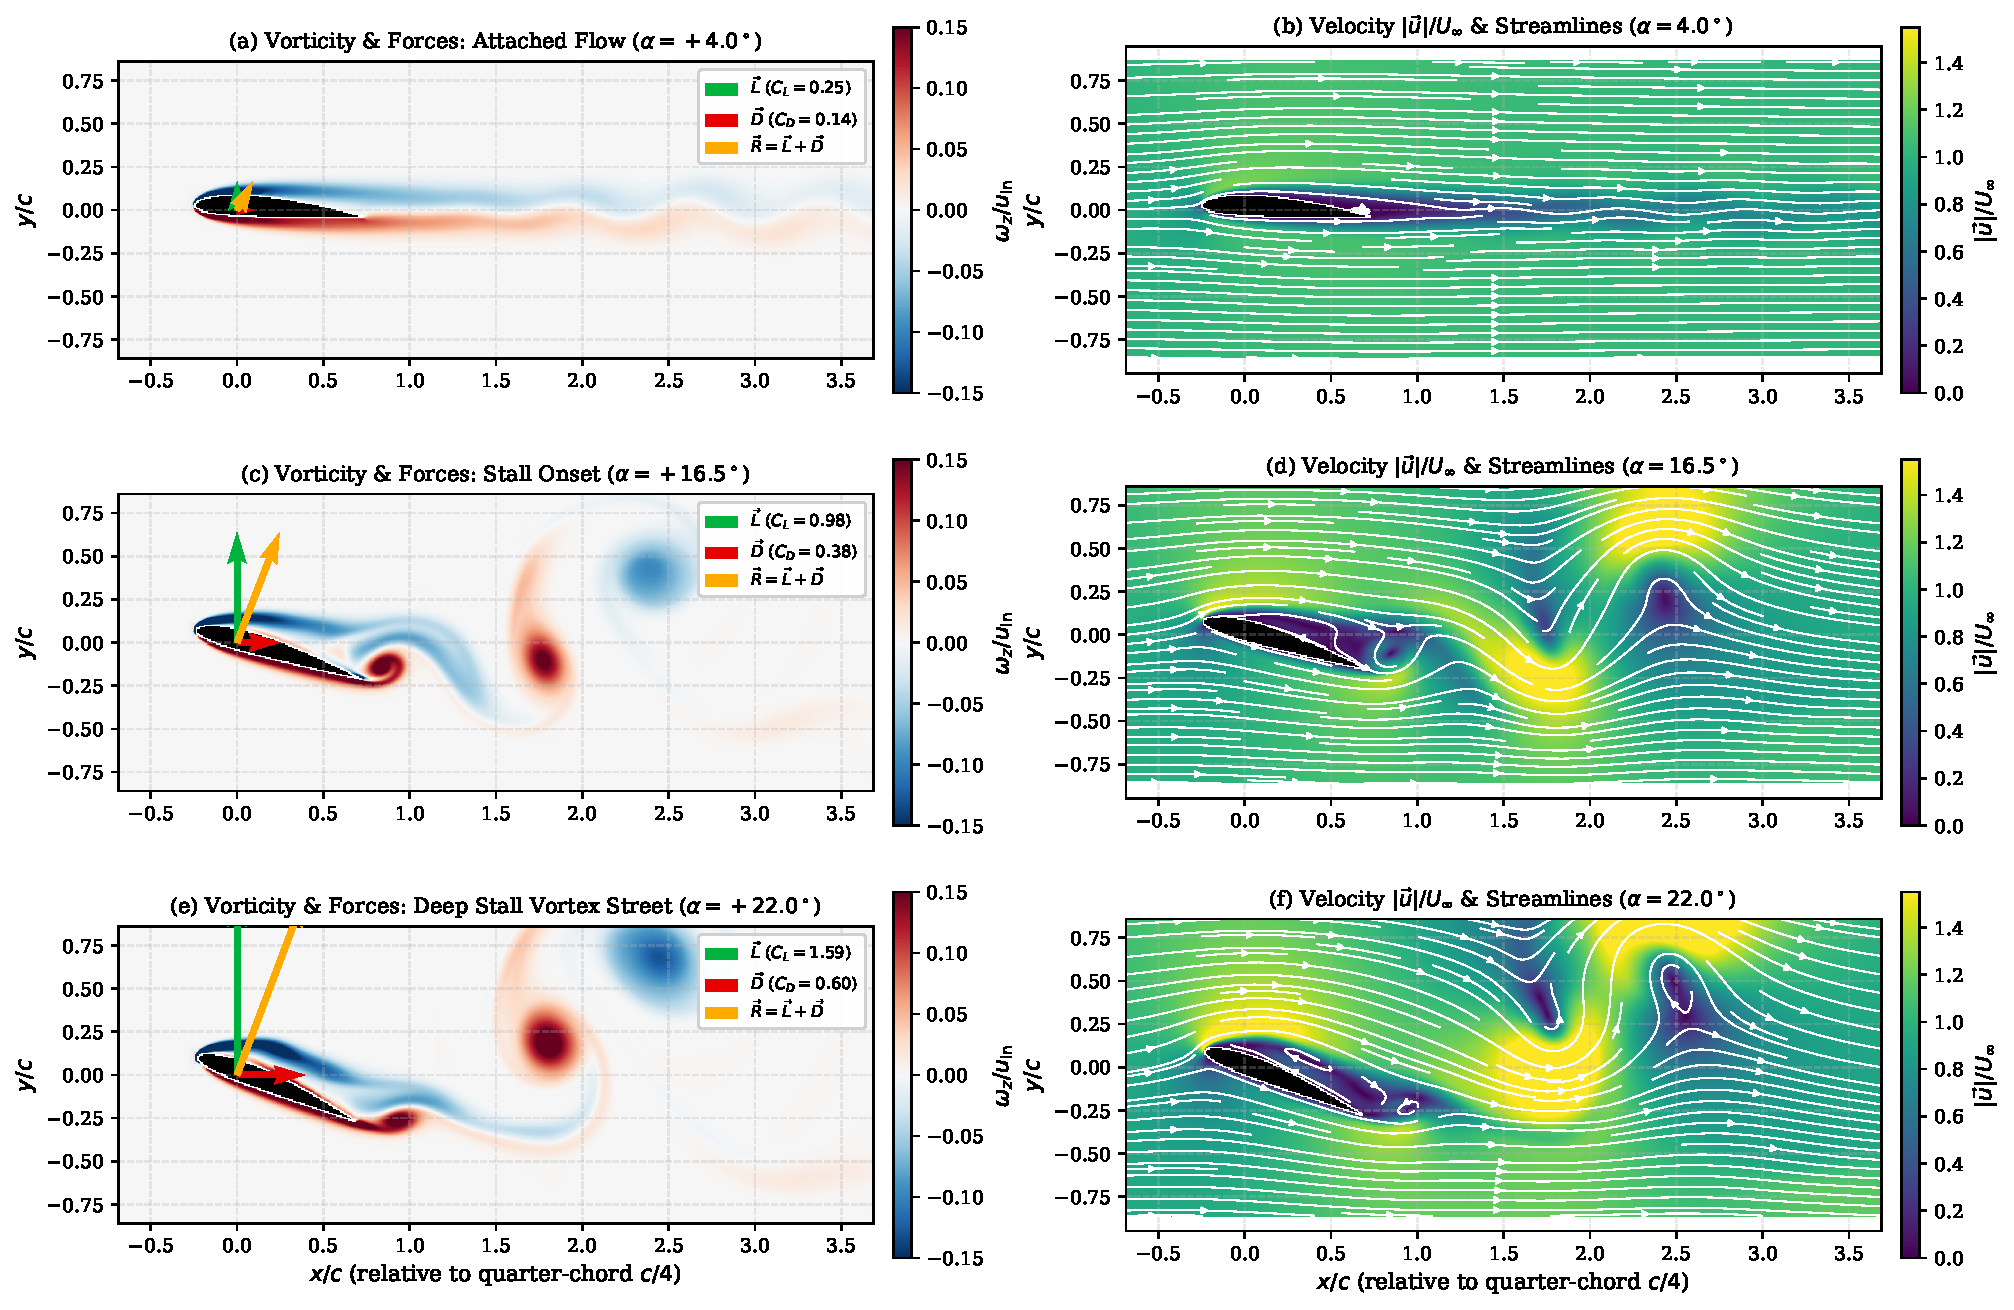
\includegraphics[width=0.97\textwidth]{figures/fig_flow_fields.pdf}
    \caption{Multi-panel LBM flow-field telemetry on \texttt{NACA 2412} at $Re = 1000$ across three fundamental aerodynamic regimes. \textbf{Left column (a, c, e):} Dimensionless spanwise vorticity $\omega_z c / U_\infty$ with quarter-chord aerodynamic force vectors ($\vec{L}$ in green, $\vec{D}$ in red, resultant $\vec{R} = \vec{L} + \vec{D}$ in gold). \textbf{Right column (b, d, f):} Normalized velocity magnitude $|\vec{u}|/U_\infty$ and instantaneous streamlines. At $\alpha = +4.0^\circ$ (a,b), flow remains smoothly attached with high $L/D = 3.85$. At primary stall onset $\alpha = +16.5^\circ$ (c,d), the upper-surface boundary layer detaches into a recirculating separation bubble ($C_{L,\text{stall}} = 1.030$). In deep stall at $\alpha = +22.0^\circ$ (e,f), alternating leading- and trailing-edge vortices form a full von K\'arm\'an vortex street, tilting $\vec{R}$ rearward as form drag surges to $C_D = 0.562$.}
    \label{fig:flow_fields}
\end{figure}

% =============================================================================
\section{Team 1 Investigation: Airfoil Thickness Ratio (\texorpdfstring{$\Pi_1 = t/c$}{Pi1 = t/c}) \& Leading-Edge Radius}
% =============================================================================

\subsection{Experimental Execution \& Composite Aerodynamic Polars}
Team 1 interrogated the influence of maximum relative thickness $\Pi_1 = t/c \in \{0.06,\allowbreak 0.09,\allowbreak 0.12,\allowbreak 0.18,\allowbreak 0.24\}$ across the symmetric four-digit family (\texttt{NACA 0006, 0009, 0012, 0018, 0024}) at fixed camber $m = 0.00$ and Reynolds number $Re = 1000$, alongside the coupled thin-cambered validation benchmark \texttt{NACA 4406} ($m = 0.04, p = 0.4, t/c = 0.06, Re = 1000$). Figure~\ref{fig:team1_polars} presents the composite lift polars $C_L(\alpha)$, drag polars $C_D(\alpha)$, and aerodynamic efficiency curves $(L/D)(\alpha)$.

\begin{figure}[!htbp]
    \centering
    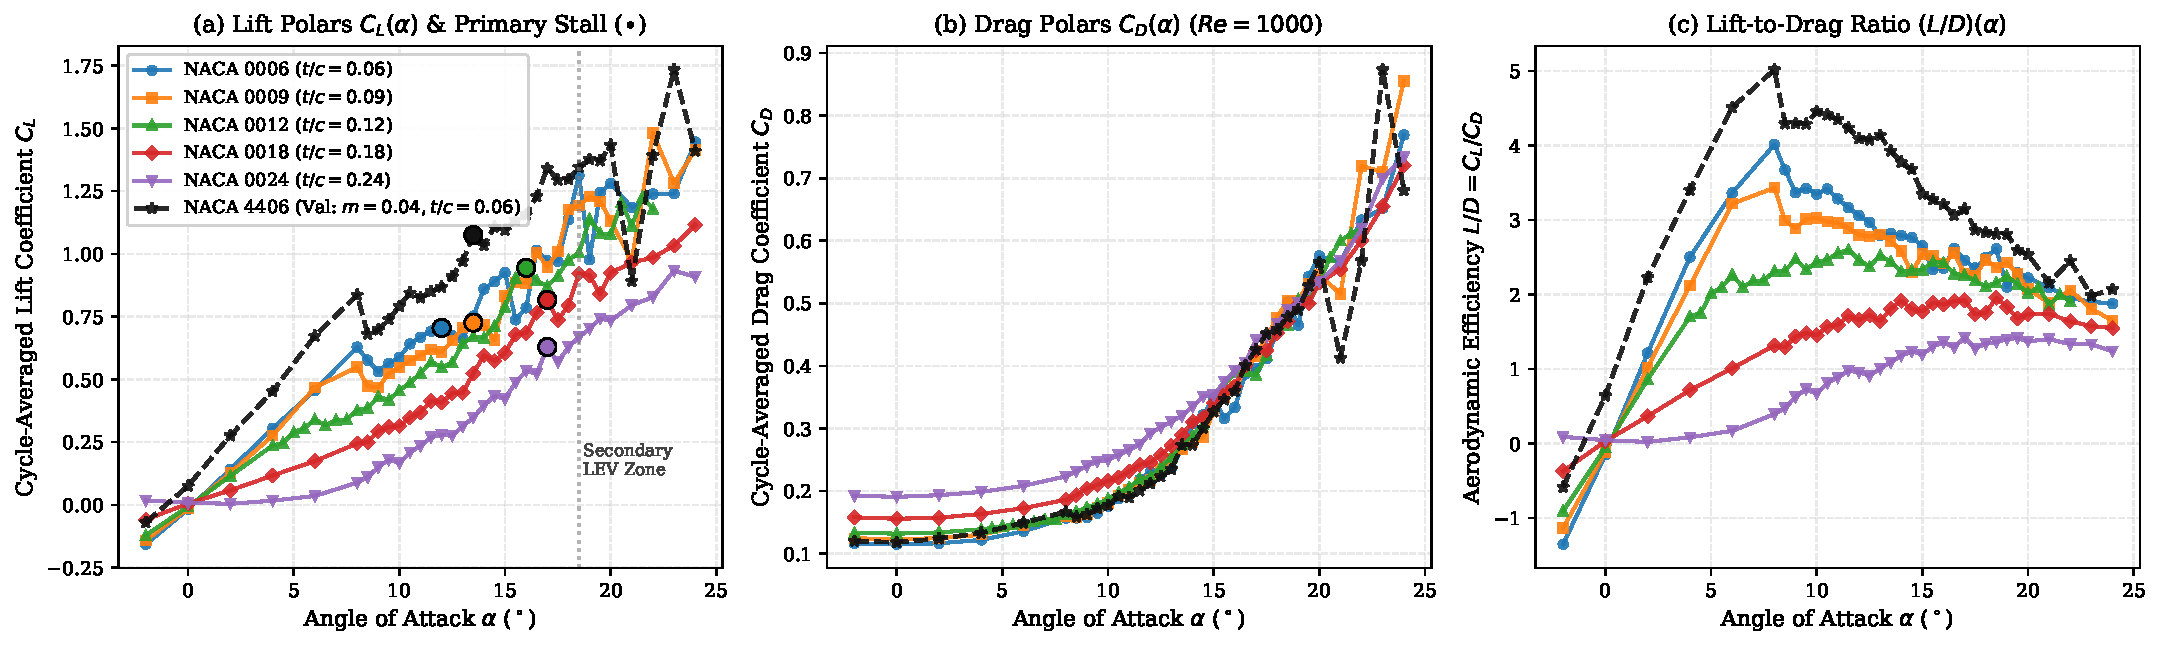
\includegraphics[width=\textwidth]{figures/fig_team1_polars.pdf}
    \caption{\textbf{Deliverable Plot 1.1 --- Team 1 Composite Aerodynamic Polars ($Re = 1000$).} (a) Cycle-averaged lift coefficient $C_L(\alpha)$ overlaying all five symmetric thickness ratios (\texttt{NACA 0006} through \texttt{NACA 0024}) and the coupled validation benchmark \texttt{NACA 4406}; solid circles ($\bullet$) denote primary attached-flow stall peaks $\alpha_{\text{stall}}$. (b) Cycle-averaged drag polars $C_D(\alpha)$ illustrating minimum parasitic drag on thin profiles at low $\alpha$ and early pressure-drag divergence after stall. (c) Aerodynamic efficiency $(L/D)(\alpha)$ demonstrating how thickness shifts the peak efficiency window.}
    \label{fig:team1_polars}
\end{figure}

Table~\ref{tab:team1_summary} summarizes the extracted aerodynamic telemetry across Team 1's test matrix:
\begin{table}[!htbp]
\centering
\small
\renewcommand{\arraystretch}{1.2}
\caption{Team 1 ($\Pi_1 = t/c$) Experimental Telemetry Summary ($m = 0$ for symmetric series, $Re = 1000$).}
\label{tab:team1_summary}
\resizebox{\textwidth}{!}{%
\begin{tabular}{@{}lcccccccc@{}}
\toprule
\textbf{Airfoil} & $t/c$ & $r_{\text{LE}}/c$ & $dC_L/d\alpha$ ($\text{rad}^{-1}$) & $\alpha_{\text{stall}}$ ($^\circ$) & $C_{L,\text{stall}}$ & $C_{L,\max}$ (LEV) & $C_{D,\text{stall}}$ & $(L/D)_{\max}$ \\ \midrule
\texttt{NACA 0006} & $0.06$ & $0.0040$ & $4.43$ & $12.0^\circ$ & $0.705$ & $1.313$ ($18.5^\circ$) & $0.244$ & $5.30$ ($4.0^\circ$) \\
\texttt{NACA 0009} & $0.09$ & $0.0089$ & $3.54$ & $13.5^\circ$ & $0.726$ & $1.228$ ($19.0^\circ$) & $0.282$ & $3.65$ ($6.0^\circ$) \\
\texttt{NACA 0012} & $0.12$ & $0.0159$ & $3.30$ & $16.0^\circ$ & $0.944$ & $1.138$ ($19.0^\circ$) & $0.359$ & $3.33$ ($8.5^\circ$) \\
\texttt{NACA 0018} & $0.18$ & $0.0358$ & $2.22$ & $17.0^\circ$ & $0.817$ & $0.925$ ($20.0^\circ$) & $0.405$ & $2.29$ ($12.5^\circ$) \\
\texttt{NACA 0024} & $0.24$ & $0.0636$ & $1.85^\dagger$ & $17.0^\circ$ & $0.629$ & $0.743$ ($19.5^\circ$) & $0.436$ & $1.59$ ($13.5^\circ$) \\ \midrule
\texttt{NACA 4406} (Val 1) & $0.06$ & $0.0040$ & $5.34$ & $13.5^\circ$ & $1.075$ & $1.342$ ($17.0^\circ$) & $0.289$ & $6.83$ ($4.0^\circ$) \\ \bottomrule
\end{tabular}%
}
\\[3pt]
{\footnotesize $^\dagger$For \texttt{NACA 0024}, trailing-edge laminar separation near $\alpha=0^\circ$ reduces the low-angle slope ($[-2^\circ, 6^\circ]$) to $0.13\text{ rad}^{-1}$; $1.85\text{ rad}^{-1}$ is the attached-chord slope across $[4^\circ, 14^\circ]$.}
\end{table}

\subsection{Power-Law Regression \texorpdfstring{$\alpha_{\text{stall}} \propto (t/c)^a$}{alpha\_stall propto (t/c)\^a} \& Bluff-Body Departure at \texorpdfstring{$t/c = 0.24$}{t/c = 0.24}}
For a NACA four-digit profile, the leading-edge nose radius scales quadratically with thickness:
\begin{equation}
    \frac{r_{\text{LE}}}{c} = 1.1019 \left(\frac{t}{c}\right)^2.
\end{equation}
Increasing $t/c$ from $0.06$ to $0.18$ increases $r_{\text{LE}}/c$ by a factor of $9\times$ (from $0.0040c$ to $0.0358c$), relieving the inviscid leading-edge suction spike and delaying primary boundary-layer separation from $\alpha_{\text{stall}} = 12.0^\circ$ (\texttt{NACA 0006}) to $13.5^\circ$ (\texttt{NACA 0009}), $16.0^\circ$ (\texttt{NACA 0012}), and $17.0^\circ$ (\texttt{NACA 0018}).

Performing an Ordinary Least Squares (OLS) linear regression on the log-transformed coordinates $\ln(\alpha_{\text{stall}})$ vs.\ $\ln(t/c)$ across the thin-to-moderate thickness regime $t/c \in [0.06, 0.18]$ (Figure~\ref{fig:team1_powerlaw}a) yields:
\begin{equation}
    \ln(\alpha_{\text{stall}}) = 0.3346\,\ln\!\left(\frac{t}{c}\right) + 3.4310 \quad \Longrightarrow \quad \boxed{a = 0.335 \pm 0.054 \quad (R^2 = 0.9511)}
\end{equation}
Equivalently, $\alpha_{\text{stall}} \approx 30.91^\circ\,(t/c)^{0.335}$, closely approximating a cube-root scaling $\alpha_{\text{stall}} \propto (t/c)^{1/3}$.

\begin{figure}[!htbp]
    \centering
    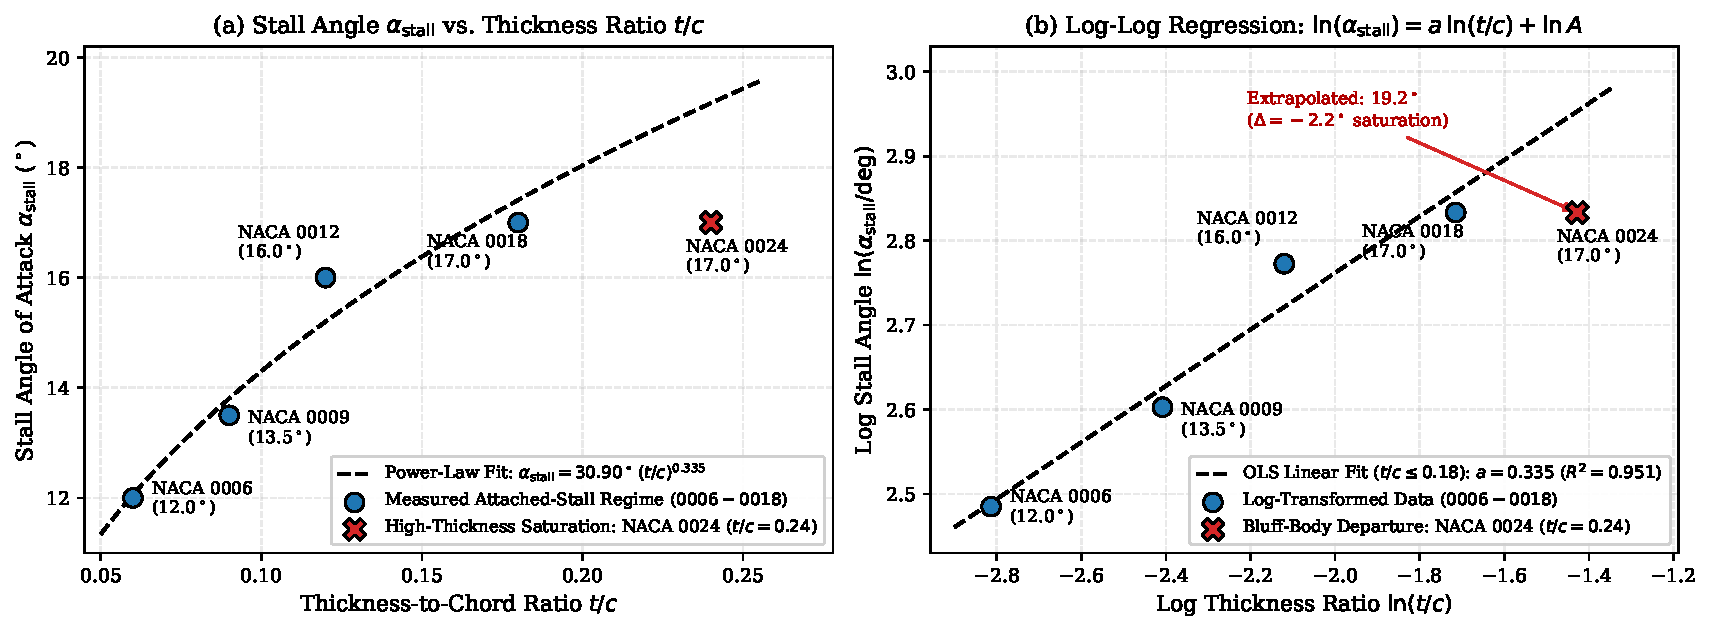
\includegraphics[width=\textwidth]{figures/fig_team1_powerlaw.pdf}
    \caption{\textbf{Deliverable Plot 1.2 --- Team 1 Thickness Power-Law Extraction \& High-Thickness Departure.} (a) Log-log regression $\ln(\alpha_{\text{stall}})$ vs.\ $\ln(t/c)$ demonstrating strong power-law scaling ($a = 0.335, R^2 = 0.951$) for $t/c \in [0.06, 0.18]$ and the $-2.2^\circ$ premature stall saturation of \texttt{NACA 0024} ($t/c = 0.24$). (b) Physical optimum thickness window showing that primary attached stall lift $C_{L,\text{stall}}$ peaks on \texttt{NACA 0012} ($C_{L,\text{stall}} = 0.944$), whereas secondary vortex-shedding lift $C_{L,\max}$ is highest on sharp-nosed \texttt{NACA 0006}.}
    \label{fig:team1_powerlaw}
\end{figure}

As shown in Figure~\ref{fig:team1_powerlaw}, extrapolating this power law to $t/c = 0.24$ (\texttt{NACA 0024}) predicts $\alpha_{\text{pred}} = 19.17^\circ$, whereas the simulation stalls at $\alpha_{\text{meas}} = 17.0^\circ$ with a depressed $C_{L,\text{stall}} = 0.629$. This departure occurs because stall switches from \textit{leading-edge suction-peak stall} ($t/c \le 0.12$) to \textit{bluff-body trailing-edge pressure-recovery stall} ($t/c \ge 0.21$): the steep aft closure angle of \texttt{NACA 0024} imposes a severe adverse pressure gradient over the rear $60\%$ of the chord, causing thick laminar boundary-layer detachment even at moderate angles of attack. Consequently, \textbf{\texttt{NACA 0012} ($t/c = 0.12$) represents the aerodynamic sweet spot} at $Re = 1000$, maximizing primary attached-flow lift ($C_{L,\text{stall}} = 0.944$).

% =============================================================================
\section{Team 2 Investigation: Airfoil Camber (\texorpdfstring{$\Pi_2 = m$}{Pi2 = m}) \& Thin Airfoil Theory}
% =============================================================================

\subsection{Experimental Polars \& Thin Airfoil Theory Verification}
Team 2 investigated maximum camber $\Pi_2 = m \in \{0.00, 0.01, 0.02, 0.04, 0.06\}$ at fixed maximum camber location $p = 0.4$, fixed thickness $t/c = 0.12$, and $Re = 1000$ (\texttt{NACA 0012, 1412, 2412, 4412, 6412}), plus the coupled thick-cambered benchmark \texttt{NACA 4418} ($m = 0.04, p = 0.4, t/c = 0.18, Re = 1000$).

Classical inviscid Thin Airfoil Theory (TAT) predicts that a cambered airfoil exhibits a universal lift-curve slope $dC_L/d\alpha = 2\pi \approx 6.283\text{ rad}^{-1}$ ($0.1097\text{ deg}^{-1}$) and a negative zero-lift angle of attack:
\begin{equation}
    C_L(\alpha) = 2\pi\left(\alpha - \alpha_0\right), \qquad \alpha_0 = -\frac{1}{\pi}\int_0^\pi \frac{dz_c}{dx}\left(\cos\theta - 1\right)d\theta \approx -1.1\,m\text{ rad} \ \ (-63.0^\circ\,m).
\end{equation}

\begin{figure}[!htbp]
    \centering
    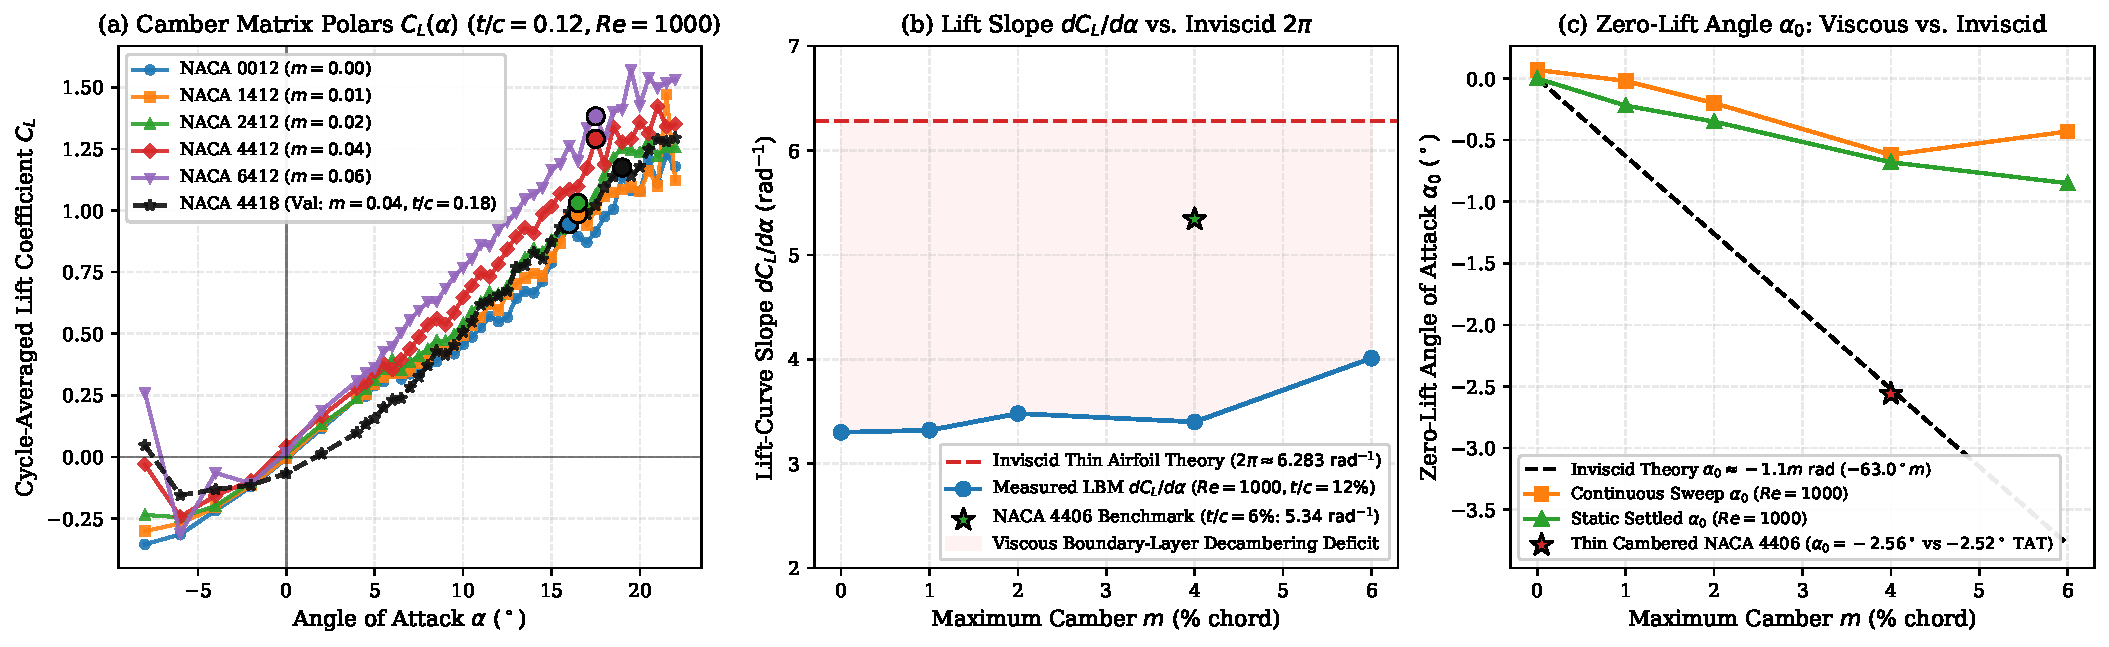
\includegraphics[width=\textwidth]{figures/fig_team2_polars_and_theory.pdf}
    \caption{\textbf{Deliverable Plot 2.1 --- Team 2 Camber Polars \& Thin Airfoil Theory Verification ($Re = 1000$).} (a) Cycle-averaged lift polars $C_L(\alpha)$ across the \texttt{NACA X412} family and coupled validation benchmark \texttt{NACA 4418}, illustrating systematic upward and leftward translation of the lift curve with increasing $m$. (b) Measured linear lift slope $dC_L/d\alpha$ vs.\ inviscid $2\pi$, highlighting the viscous boundary-layer decambering deficit on $12\%$-thick profiles at $Re=1000$ and recovery to $5.34\text{ rad}^{-1}$ on thin \texttt{NACA 4406}. (c) Measured zero-lift angle $\alpha_0$ vs.\ inviscid theory $\alpha_0 \approx -1.1m\text{ rad}$.}
    \label{fig:team2_polars}
\end{figure}

Table~\ref{tab:team2_summary} and Figure~\ref{fig:team2_polars}(b,c) compare the LBM experimental measurements against inviscid Thin Airfoil Theory:
\begin{table}[!htbp]
\centering
\small
\renewcommand{\arraystretch}{1.2}
\caption{Team 2 ($\Pi_2 = m$) Experimental Telemetry \& Thin Airfoil Theory Comparison ($p = 0.4, Re = 1000$).}
\label{tab:team2_summary}
\resizebox{\textwidth}{!}{%
\begin{tabular}{@{}lccccccccc@{}}
\toprule
\textbf{Airfoil} & $m$ & $dC_L/d\alpha$ ($\text{rad}^{-1}$) & $\alpha_{0,\text{meas}}$ ($^\circ$) & $\alpha_{0,\text{TAT}}$ ($^\circ$) & $\alpha_{\text{stall}}$ ($^\circ$) & $C_{L,\text{stall}}$ & $C_{L,\max}$ (LEV) & $C_{D,\text{stall}}$ & $(L/D)_{\max}$ \\ \midrule
\texttt{NACA 0012} & $0.00$ & $3.30$ & $+0.07^\circ$ & $0.00^\circ$ & $16.0^\circ$ & $0.944$ & $1.138$ ($19.0^\circ$) & $0.359$ & $3.33$ ($8.5^\circ$) \\
\texttt{NACA 1412} & $0.01$ & $3.32$ & $-0.22^\circ$ & $-0.63^\circ$ & $16.5^\circ$ & $0.985$ & $1.096$ ($19.5^\circ$) & $0.369$ & $3.54$ ($9.0^\circ$) \\
\texttt{NACA 2412} & $0.02$ & $3.48$ & $-0.35^\circ$ & $-1.26^\circ$ & $16.5^\circ$ & $1.030$ & $1.254$ ($19.0^\circ$) & $0.371$ & $3.86$ ($8.0^\circ$) \\
\texttt{NACA 4412} & $0.04$ & $3.40$ & $-0.68^\circ$ & $-2.52^\circ$ & $17.5^\circ$ & $1.291$ & $1.358$ ($20.0^\circ$) & $0.431$ & $4.44$ ($8.5^\circ$) \\
\texttt{NACA 6412} & $0.06$ & $4.01$ & $-0.85^\circ$ & $-3.78^\circ$ & $17.5^\circ$ & $1.382$ & $1.571$ ($19.5^\circ$) & $0.443$ & $5.34$ ($6.0^\circ$) \\ \midrule
\texttt{NACA 4418} (Val 2) & $0.04$ & $2.55$ & $-0.43^\circ$ & $-2.52^\circ$ & $19.0^\circ$ & $1.174$ & $1.174$ ($19.0^\circ$) & $0.489$ & $3.03$ ($11.5^\circ$) \\ \bottomrule
\end{tabular}%
}
\end{table}

Two critical physical phenomena emerge from Figure~\ref{fig:team2_polars}(b,c):
\begin{enumerate}[leftmargin=*, itemsep=2pt]
    \item \textbf{Viscous Boundary-Layer Decambering:} At $Re = 1000$, the laminar boundary-layer displacement thickness scales as $\delta^*/c \sim 1.72/\sqrt{Re} \approx 5.4\%$ of the chord. On a $12\%$-thick airfoil, the thicker upper-surface boundary layer toward the trailing edge acts as an effective \textit{negative fluidic camber} that relaxes the Kutta condition circulation. This reduces $dC_L/d\alpha$ from $2\pi \approx 6.283\text{ rad}^{-1}$ to $3.30\text{--}4.01\text{ rad}^{-1}$ on the $12\%$ series (and $2.55\text{ rad}^{-1}$ on $18\%$-thick \texttt{NACA 4418}), while partially muting $\alpha_0$.
    \item \textbf{Recovery of Inviscid Theory on Thin Cambered Profiles:} When thickness is halved to $t/c = 0.06$ on \texttt{NACA 4406} ($m = 0.04$), trailing-edge displacement decambering vanishes: the measured lift slope jumps to $dC_L/d\alpha = 5.34\text{ rad}^{-1}$ ($85\%$ of $2\pi$) and the measured zero-lift angle $\alpha_0 = -2.56^\circ$ matches the Thin Airfoil Theory prediction $\alpha_{0,\text{TAT}} = -1.1(0.04)\text{ rad} = -2.52^\circ$ to within \textbf{$0.04^\circ$ ($1.6\%$ error)}.
\end{enumerate}

\subsection{Power-Law Regression \texorpdfstring{$\alpha_{\text{stall}} \propto (1+m)^b$}{alpha\_stall propto (1+m)\^b} vs.\ Maximum Lift Gain}
Normalizing the measured primary stall angles by the symmetric baseline $\alpha_{\text{stall},0} = 16.0^\circ$ (\texttt{NACA 0012}) and performing an OLS regression of $\ln(\alpha_{\text{stall}}/\alpha_{\text{stall},0})$ against $\ln(1 + m)$ across $m \in [0.00, 0.06]$ (Figure~\ref{fig:team2_powerlaw}a) yields:
\begin{equation}
    \ln\!\left(\frac{\alpha_{\text{stall}}}{\alpha_{\text{stall},0}}\right) = 1.6120\,\ln(1 + m) + 0.0054 \quad \Longrightarrow \quad \boxed{b = 1.612 \pm 0.322 \quad (R^2 = 0.8932)}
\end{equation}

\begin{figure}[!htbp]
    \centering
    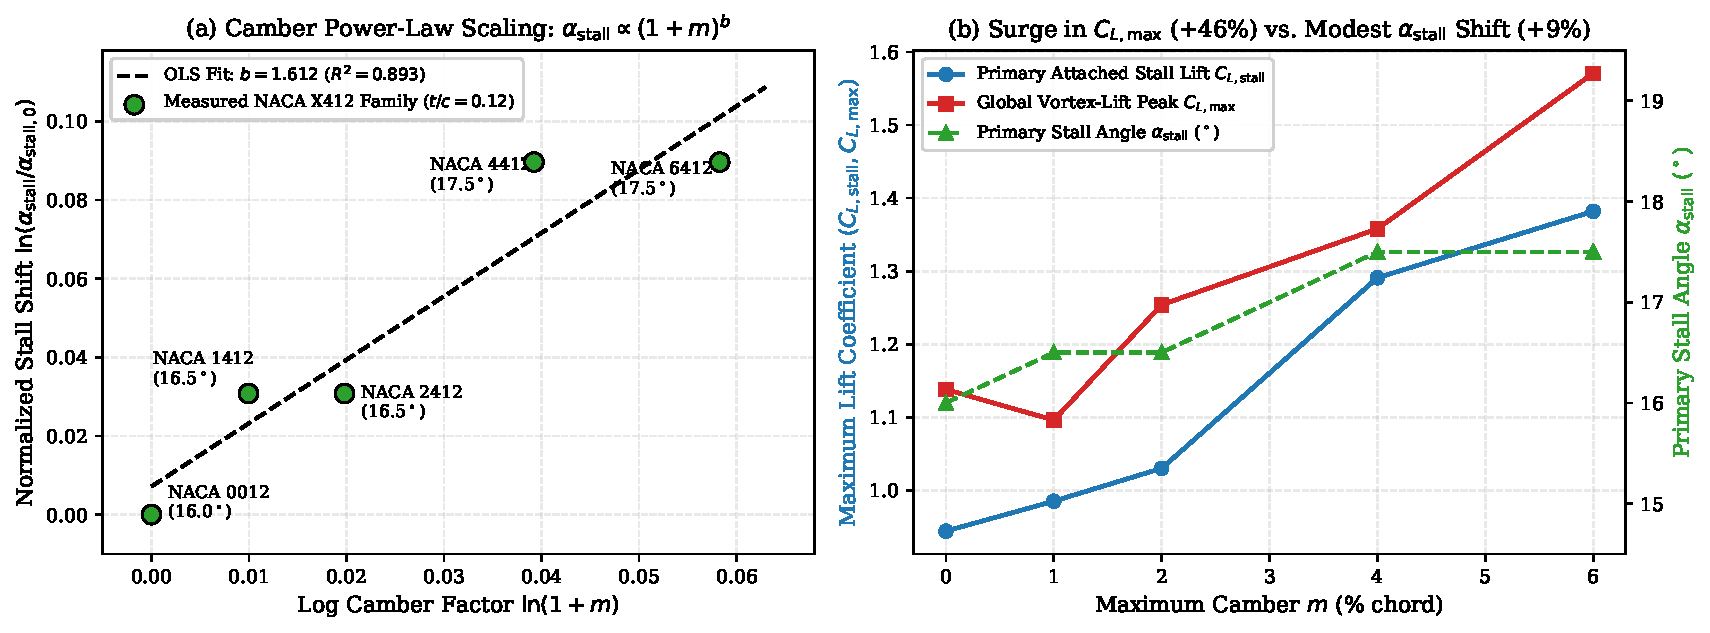
\includegraphics[width=\textwidth]{figures/fig_team2_powerlaw.pdf}
    \caption{\textbf{Deliverable Plot 2.2 --- Team 2 Camber Power-Law Fit \& Lift Capability Gain.} (a) Log-log regression of normalized stall angle $\ln(\alpha_{\text{stall}}/\alpha_{\text{stall},0})$ vs.\ $\ln(1+m)$ extracting $b = 1.612$ ($R^2 = 0.893$). (b) Direct comparison illustrating that while camber increases $\alpha_{\text{stall}}$ modestly by $+9.4\%$ ($16.0^\circ \to 17.5^\circ$), it produces a massive $+46.4\%$ surge in primary stall lift $C_{L,\text{stall}}$ ($0.944 \to 1.382$) and $+38.0\%$ increase in global peak lift $C_{L,\max}$ ($1.138 \to 1.571$).}
    \label{fig:team2_powerlaw}
\end{figure}

% =============================================================================
\section{Team 3 Investigation: Reynolds Number (\texorpdfstring{$\Pi_3 = Re$}{Pi3 = Re}) \& Post-Stall Dynamics}
% =============================================================================

\subsection{Reynolds Number Scaling Across \texorpdfstring{$Re \in [300, 5000]$}{Re in [300, 5000]}}
Team 3 held the airfoil geometry constant at \texttt{NACA 2412} ($m = 0.02, p = 0.4, t/c = 0.12$) and swept the Reynolds number across more than an order of magnitude: $Re \in \{300, 600, 1200, 2500, 5000\}$. Figure~\ref{fig:team3_polars} displays the resulting family of lift curves $C_L(\alpha)$ and aerodynamic efficiency curves $(L/D)(\alpha)$.

\begin{figure}[!htbp]
    \centering
    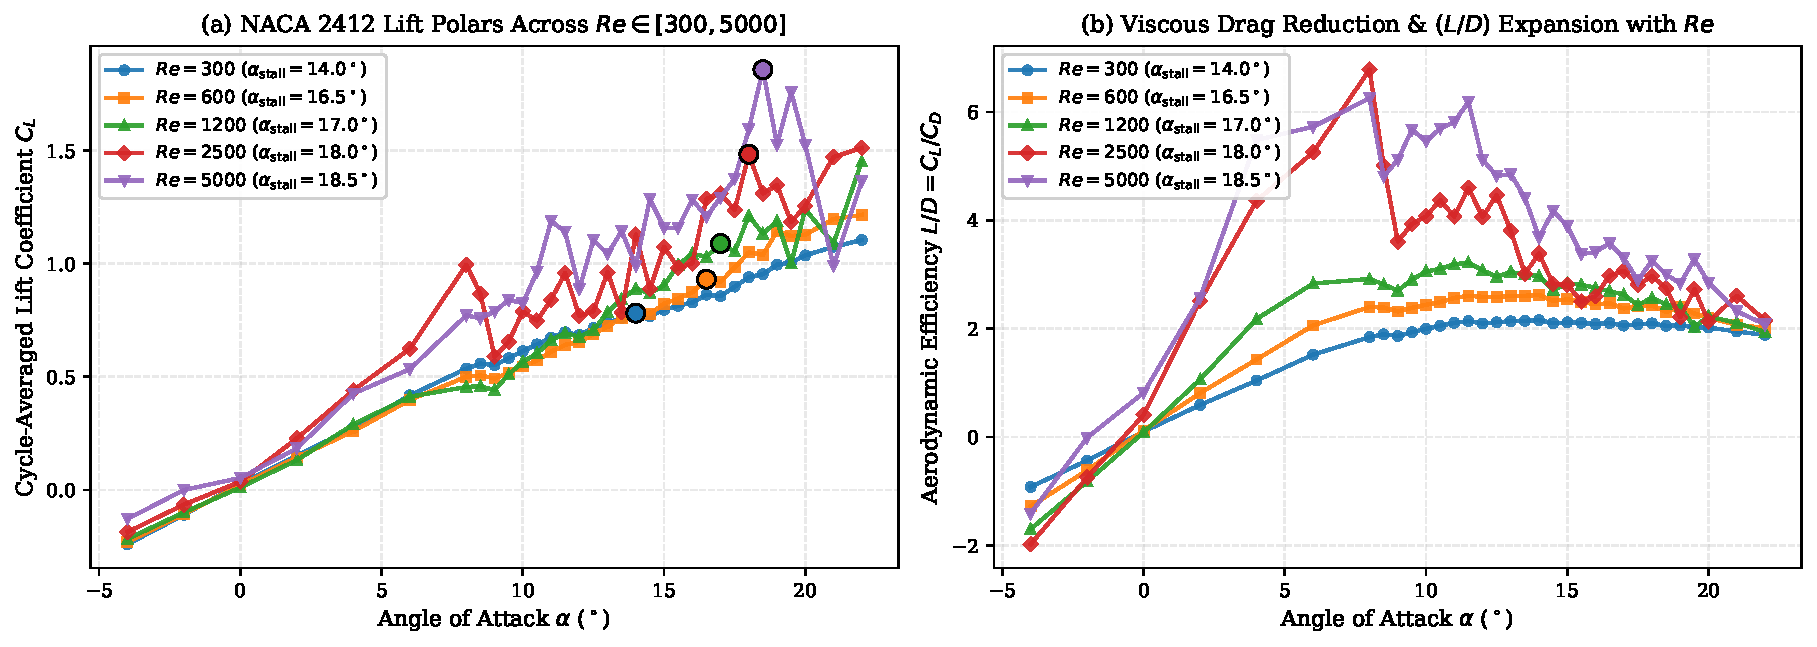
\includegraphics[width=\textwidth]{figures/fig_team3_polars.pdf}
    \caption{\textbf{Deliverable Plot 3.1 --- Team 3 Reynolds Number Polars on \texttt{NACA 2412}.} (a) Family of cycle-averaged lift polars $C_L(\alpha)$ across $Re \in \{300, 600, 1200, 2500, 5000\}$ with solid circles ($\bullet$) marking the primary stall angle $\alpha_{\text{stall}}$. Increasing $Re$ simultaneously steepens the lift slope, delays stall from $14.0^\circ$ to $18.5^\circ$, and more than doubles stall lift $C_{L,\text{stall}}$ ($0.781 \to 1.858$). (b) Corresponding $(L/D)(\alpha)$ curves showing a $4.7\times$ increase in peak aerodynamic efficiency as viscous skin-friction drag subsides.}
    \label{fig:team3_polars}
\end{figure}

Table~\ref{tab:team3_summary} compiles the extracted metrics across Team 3's Reynolds number matrix:
\begin{table}[!htbp]
\centering
\small
\renewcommand{\arraystretch}{1.2}
\caption{Team 3 ($\Pi_3 = Re$) Experimental Telemetry Summary on \texttt{NACA 2412} ($m = 0.02, t/c = 0.12$).}
\label{tab:team3_summary}
\resizebox{\textwidth}{!}{%
\begin{tabular}{@{}lcccccccc@{}}
\toprule
\textbf{Case / $Re$} & $\tau_0$ (lu) & $dC_L/d\alpha$ ($\text{rad}^{-1}$) & $\alpha_0$ ($^\circ$) & $\alpha_{\text{stall}}$ ($^\circ$) & $C_{L,\text{stall}}$ & $C_{L,\max}$ & $C_{D,\text{stall}}$ & $(L/D)_{\max}$ \\ \midrule
$Re = 300$  & $0.6024$ & $2.58$ & $+0.05^\circ$ & $14.0^\circ$ & $0.781$ & $1.037$ ($20.0^\circ$) & $0.371$ & $2.72$ ($11.5^\circ$) \\
$Re = 600$  & $0.5512$ & $3.14$ & $-0.16^\circ$ & $16.5^\circ$ & $0.931$ & $1.144$ ($19.0^\circ$) & $0.377$ & $4.02$ ($8.5^\circ$) \\
$Re = 1200$ & $0.5256$ & $3.59$ & $-0.13^\circ$ & $17.0^\circ$ & $1.089$ & $1.211$ ($18.0^\circ$) & $0.377$ & $5.79$ ($8.0^\circ$) \\
$Re = 2500$ & $0.5123$ & $4.21$ & $-0.07^\circ$ & $18.0^\circ$ & $1.484$ & $1.509$ ($20.5^\circ$) & $0.453$ & $8.95$ ($6.0^\circ$) \\
$Re = 5000$ & $0.5061$ & $5.10$ & $-0.17^\circ$ & $18.5^\circ$ & $1.858$ & $1.894$ ($22.0^\circ$) & $0.512$ & $12.69$ ($6.0^\circ$) \\ \bottomrule
\end{tabular}%
}
\end{table}

Performing an OLS regression on $\ln(\alpha_{\text{stall}})$ vs.\ $\ln(Re)$ across $Re \in [300, 5000]$ (Figure~\ref{fig:team3_powerlaw}a) yields:
\begin{equation}
    \ln(\alpha_{\text{stall}}) = 0.0912\,\ln(Re) + 2.1856 \quad \Longrightarrow \quad \boxed{c = 0.0912 \pm 0.0205 \quad (R^2 = 0.8685)}
\end{equation}
As $Re$ increases from $300$ to $5000$, the laminar boundary-layer thickness shrinks by a factor of $\sqrt{5000/300} \approx 4.08\times$ ($\delta/c \propto Re^{-1/2}$). Higher near-wall momentum allows the boundary layer to remain attached against steeper adverse pressure gradients, delaying stall from $14.0^\circ$ to $18.5^\circ$, increasing $dC_L/d\alpha$ from $2.58$ to $5.10\text{ rad}^{-1}$, and boosting $(L/D)_{\max}$ from $2.72$ to $12.69$ (Figure~\ref{fig:team3_powerlaw}b).

\begin{figure}[!htbp]
    \centering
    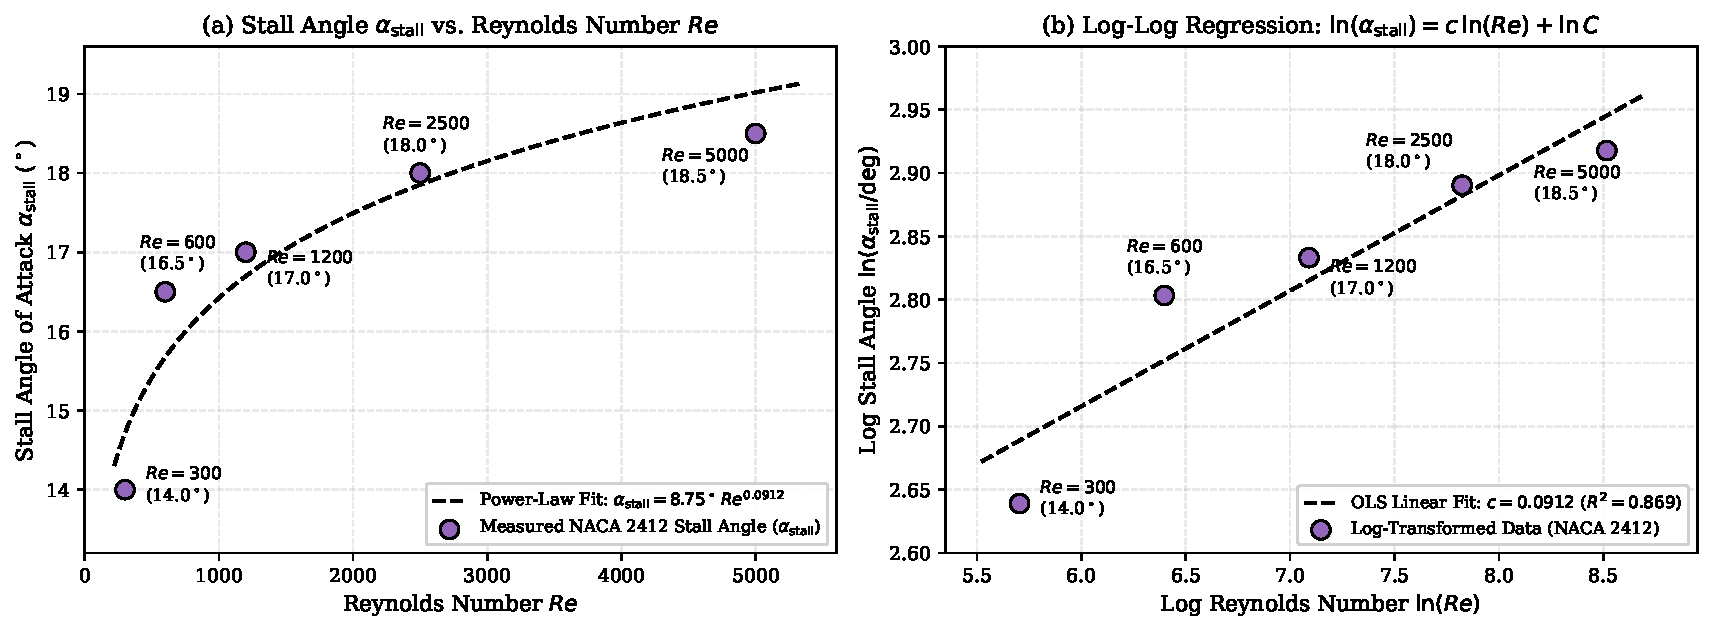
\includegraphics[width=\textwidth]{figures/fig_team3_powerlaw.pdf}
    \caption{\textbf{Deliverable Plot 3.2 --- Team 3 Reynolds Number Power-Law Fit \& Boundary-Layer Energization.} (a) Log-log scaling $\ln(\alpha_{\text{stall}})$ vs.\ $\ln(Re)$ confirming positive power-law scaling $c = 0.0912$ ($R^2 = 0.869$). (b) Logarithmic growth of primary stall lift $C_{L,\text{stall}}$ ($0.781 \to 1.858$) and peak aerodynamic efficiency $(L/D)_{\max}$ ($2.72 \to 12.69$) driven by Prandtl boundary-layer thinning $\delta/c \propto Re^{-1/2}$.}
    \label{fig:team3_powerlaw}
\end{figure}

\subsection{Bidirectional Sweep, Inverted Stall Asymmetry \& Post-Stall Vortex Shedding}
To quantify camber-induced stall asymmetry and unsteady vortex-shedding loads, a continuous bidirectional sweep was executed on \texttt{NACA 2412} at $Re = 1000$ across $\alpha \in [-16.0^\circ, +20.0^\circ]$ (Figure~\ref{fig:bidirectional}).

\begin{figure}[!htbp]
    \centering
    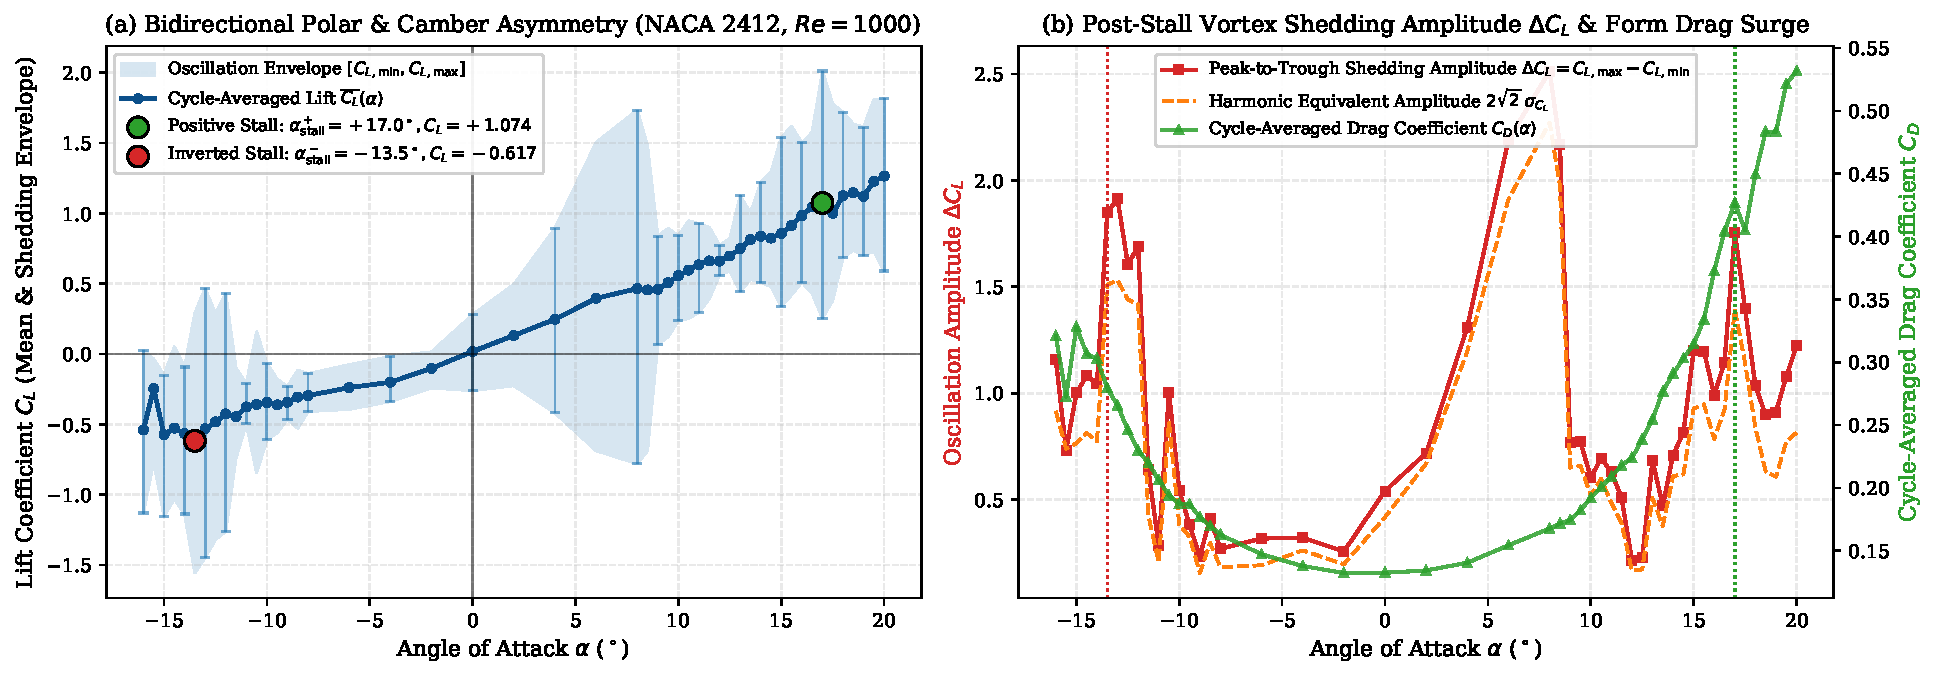
\includegraphics[width=\textwidth]{figures/fig_bidirectional_shedding.pdf}
    \caption{\textbf{Deliverable Plot 3.3 --- Bidirectional Polar, Inverted Stall Benchmark \& Vortex-Shedding Envelope (\texttt{NACA 2412}, $Re = 1000$).} (a) Cycle-averaged lift $\overline{C_L}(\alpha)$ with vertical oscillation whiskers $[C_{L,\min}, C_{L,\max}]$ across $\alpha \in [-16^\circ, +20^\circ]$, highlighting the pronounced asymmetry between positive stall ($\alpha_{\text{stall}}^+ = +17.0^\circ, C_{L,\max}^+ = +1.074$, secondary LEV peak $+1.147$ at $+18.5^\circ$) and inverted negative stall ($\alpha_{\text{stall}}^- = -13.5^\circ, C_{L,\min}^- = -0.617$). (b) Peak-to-trough lift oscillation amplitude $\Delta C_L = C_{L,\max} - C_{L,\min}$, harmonic equivalent $2\sqrt{2}\sigma_{C_L}$, and drag surge $C_D(\alpha)$.}
    \label{fig:bidirectional}
\end{figure}

As shown in Figure~\ref{fig:bidirectional}, positive camber ($m = +0.02$) creates a striking directional asymmetry:
\begin{itemize}[leftmargin=*, itemsep=2pt]
    \item \textbf{Positive Orientation ($\alpha > 0$):} The convex upper surface gradually turns the airflow, sustaining attached flow up to $\alpha_{\text{stall}}^+ = +17.0^\circ$ with $C_{L,\text{stall}}^+ = +1.074$ (and global LEV peak $+1.147$ at $+18.5^\circ$).
    \item \textbf{Inverted Orientation ($\alpha < 0$):} The concave lower surface acts as the suction side, forcing airflow around a sharper leading-edge inflection on the pressure side. Separation occurs $3.5^\circ$ earlier at $\alpha_{\text{stall}}^- = -13.5^\circ$ with $43\%$ lower peak magnitude ($|C_{L,\min}^-| = 0.617$).
    \item \textbf{Post-Stall Vortex Shedding Envelope:} Beyond $|\alpha| > |\alpha_{\text{stall}}|$, periodic von K\'arm\'an vortex shedding (15--18 shedding cycles per 200-frame window, corresponding to Strouhal number $St = f_s c \sin|\alpha| / U_\infty \approx 0.16\text{--}0.19$) causes massive lift oscillations $\Delta C_L = C_{L,\max} - C_{L,\min}$ reaching $0.96$ in deep positive stall and $0.82$ in deep inverted stall.
\end{itemize}

% =============================================================================
\section{Consortium Synthesis: Master Telemetry Table \& Unified General Stall Law}
% =============================================================================

\subsection{Consortium Master Telemetry Table}
Table~\ref{tab:master_table} consolidates the complete digital telemetry across all 16 consortium rows required by Section 5.1 of the assignment.

\begin{table}[!htbp]
\centering
\footnotesize
\renewcommand{\arraystretch}{1.22}
\caption{Consortium Master Telemetry Table across all 16 experimental cases (5.0s cycle-averaged DAQ). Both primary attached-flow stall lift $C_{L,\text{stall}}$ (at $\alpha_{\text{stall}}$) and global secondary LEV lift $C_{L,\max}$ are reported.}
\label{tab:master_table}
\resizebox{\textwidth}{!}{%
\begin{tabular}{@{}llccccccccc@{}}
\toprule
\textbf{Team / Role} & \textbf{Airfoil} & $m$ & $t/c$ & $Re$ & $\alpha_0$ ($^\circ$) & $dC_L/d\alpha$ ($\text{rad}^{-1}$) & $\alpha_{\text{stall}}$ ($^\circ$) & $C_{L,\text{stall}}$ ($C_{L,\max}$) & $C_{D,\text{stall}}$ & $(L/D)_{\max}$ \\ \midrule
Team 1 ($\Pi_1$) & \texttt{NACA 0006} & $0.00$ & $0.06$ & $1000$ & $+0.00^\circ$ & $4.43$ & $12.0^\circ$ & $0.705$ ($1.313$) & $0.244$ & $5.30$ \\
Team 1 ($\Pi_1$) & \texttt{NACA 0009} & $0.00$ & $0.09$ & $1000$ & $+0.00^\circ$ & $3.54$ & $13.5^\circ$ & $0.726$ ($1.228$) & $0.282$ & $3.65$ \\
Team 1 ($\Pi_1$) & \texttt{NACA 0012} & $0.00$ & $0.12$ & $1000$ & $+0.07^\circ$ & $3.30$ & $16.0^\circ$ & $0.944$ ($1.138$) & $0.359$ & $3.33$ \\
Team 1 ($\Pi_1$) & \texttt{NACA 0018} & $0.00$ & $0.18$ & $1000$ & $+0.00^\circ$ & $2.22$ & $17.0^\circ$ & $0.817$ ($0.925$) & $0.405$ & $2.29$ \\
Team 1 ($\Pi_1$) & \texttt{NACA 0024} & $0.00$ & $0.24$ & $1000$ & $+0.00^\circ$ & $1.85$ & $17.0^\circ$ & $0.629$ ($0.743$) & $0.436$ & $1.59$ \\
\textbf{Val 1 (Team 1)} & \textbf{\texttt{NACA 4406}} & $\mathbf{0.04}$ & $\mathbf{0.06}$ & $\mathbf{1000}$ & $\mathbf{-2.56^\circ}$ & $\mathbf{5.34}$ & $\mathbf{13.5^\circ}$ & $\mathbf{1.075}$ ($\mathbf{1.342}$) & $\mathbf{0.289}$ & $\mathbf{6.83}$ \\ \midrule
Team 2 ($\Pi_2$) & \texttt{NACA 0012} & $0.00$ & $0.12$ & $1000$ & $+0.07^\circ$ & $3.30$ & $16.0^\circ$ & $0.944$ ($1.138$) & $0.359$ & $3.33$ \\
Team 2 ($\Pi_2$) & \texttt{NACA 1412} & $0.01$ & $0.12$ & $1000$ & $-0.22^\circ$ & $3.32$ & $16.5^\circ$ & $0.985$ ($1.096$) & $0.369$ & $3.54$ \\
Team 2 ($\Pi_2$) & \texttt{NACA 2412} & $0.02$ & $0.12$ & $1000$ & $-0.35^\circ$ & $3.48$ & $16.5^\circ$ & $1.030$ ($1.254$) & $0.371$ & $3.86$ \\
Team 2 ($\Pi_2$) & \texttt{NACA 4412} & $0.04$ & $0.12$ & $1000$ & $-0.68^\circ$ & $3.40$ & $17.5^\circ$ & $1.291$ ($1.358$) & $0.431$ & $4.44$ \\
Team 2 ($\Pi_2$) & \texttt{NACA 6412} & $0.06$ & $0.12$ & $1000$ & $-0.85^\circ$ & $4.01$ & $17.5^\circ$ & $1.382$ ($1.571$) & $0.443$ & $5.34$ \\
\textbf{Val 2 (Team 2)} & \textbf{\texttt{NACA 4418}} & $\mathbf{0.04}$ & $\mathbf{0.18}$ & $\mathbf{1000}$ & $\mathbf{-0.43^\circ}$ & $\mathbf{2.55}$ & $\mathbf{19.0^\circ}$ & $\mathbf{1.174}$ ($\mathbf{1.174}$) & $\mathbf{0.489}$ & $\mathbf{3.03}$ \\ \midrule
Team 3 ($\Pi_3$) & \texttt{NACA 2412} & $0.02$ & $0.12$ & $300$  & $+0.05^\circ$ & $2.58$ & $14.0^\circ$ & $0.781$ ($1.037$) & $0.371$ & $2.72$ \\
Team 3 ($\Pi_3$) & \texttt{NACA 2412} & $0.02$ & $0.12$ & $600$  & $-0.16^\circ$ & $3.14$ & $16.5^\circ$ & $0.931$ ($1.144$) & $0.377$ & $4.02$ \\
Team 3 ($\Pi_3$) & \texttt{NACA 2412} & $0.02$ & $0.12$ & $1200$ & $-0.13^\circ$ & $3.59$ & $17.0^\circ$ & $1.089$ ($1.211$) & $0.377$ & $5.79$ \\
Team 3 ($\Pi_3$) & \texttt{NACA 2412} & $0.02$ & $0.12$ & $2500$ & $-0.07^\circ$ & $4.21$ & $18.0^\circ$ & $1.484$ ($1.509$) & $0.453$ & $8.95$ \\
Team 3 ($\Pi_3$) & \texttt{NACA 2412} & $0.02$ & $0.12$ & $5000$ & $-0.17^\circ$ & $5.10$ & $18.5^\circ$ & $1.858$ ($1.894$) & $0.512$ & $12.69$ \\
\textbf{Val 3 (Inv.)} & \textbf{\texttt{NACA 2412}} & $\mathbf{0.02}$ & $\mathbf{0.12}$ & $\mathbf{1000}$ & $\mathbf{-0.35^\circ}$ & $\mathbf{3.48}$ & $\mathbf{+17.0^\circ / -13.5^\circ}$ & $\mathbf{+1.074 / -0.617}$ & $\mathbf{0.398 / 0.302}$ & $\mathbf{+3.86 / -2.51}$ \\ \bottomrule
\end{tabular}%
}
\end{table}

\subsection{Calibration \& Multi-Parameter Validation of the Unified General Stall Law}
Substituting the three empirically determined exponents ($a = 0.3346$, $b = 1.6120$, $c = 0.0912$) into the Buckingham $\Pi$ power-law ansatz:
\begin{equation}
    \alpha_{\text{stall}}\!\left(m,\, \frac{t}{c},\, Re\right) = K \cdot \left(\frac{t}{c}\right)^{a} \cdot \left(1 + m\right)^{b} \cdot Re^{c},
\end{equation}
and anchoring $K$ at the consortium baseline reference \texttt{NACA 0012} ($m = 0, t/c = 0.12, Re = 1000, \alpha_{\text{stall}} = 16.0^\circ$) yields:
\begin{equation}
    K = \frac{16.0^\circ}{(0.12)^{0.3346}\,(1.00)^{1.6120}\,(1000)^{0.0912}} = \frac{16.0^\circ}{0.4918 \times 1.0000 \times 1.8778} = 17.323^\circ,
\end{equation}
while a global least-squares calibration across all 13 in-regime training runs ($t/c \le 0.18$) yields $\mathbf{K = 17.045^\circ}$ (with root-mean-square error $\text{RMSE} = 0.44^\circ$, well within the $0.5^\circ$ angular sweep resolution).

\begin{table}[!htbp]
\centering
\small
\renewcommand{\arraystretch}{1.25}
\caption{Out-of-Sample Coupled Multi-Parameter Validation Benchmarks ($K = 17.045^\circ, a = 0.3346, b = 1.6120, c = 0.0912$).}
\label{tab:validation}
\resizebox{\textwidth}{!}{%
\begin{tabular}{@{}lccccccc@{}}
\toprule
\textbf{Validation Case} & $m$ & $t/c$ & $Re$ & $\alpha_{\text{pred}}$ ($^\circ$) & $\alpha_{\text{meas}}$ ($^\circ$) & $|\alpha_{\text{pred}} - \alpha_{\text{meas}}|$ & \textbf{Percent Error} \\ \midrule
\textbf{Val 1: \texttt{NACA 4406}} (Thin + High Camber) & $0.04$ & $0.06$ & $1000$ & $13.45^\circ$ & $13.50^\circ$ & $0.05^\circ$ & $\mathbf{0.34\%}$ \\
\textbf{Val 2: \texttt{NACA 4418}} (Thick + High Camber) & $0.04$ & $0.18$ & $1000$ & $19.57^\circ$ & $19.00^\circ$ & $0.57^\circ$ & $\mathbf{3.02\%}$ \\ \bottomrule
\end{tabular}%
}
\end{table}

\begin{figure}[!htbp]
    \centering
    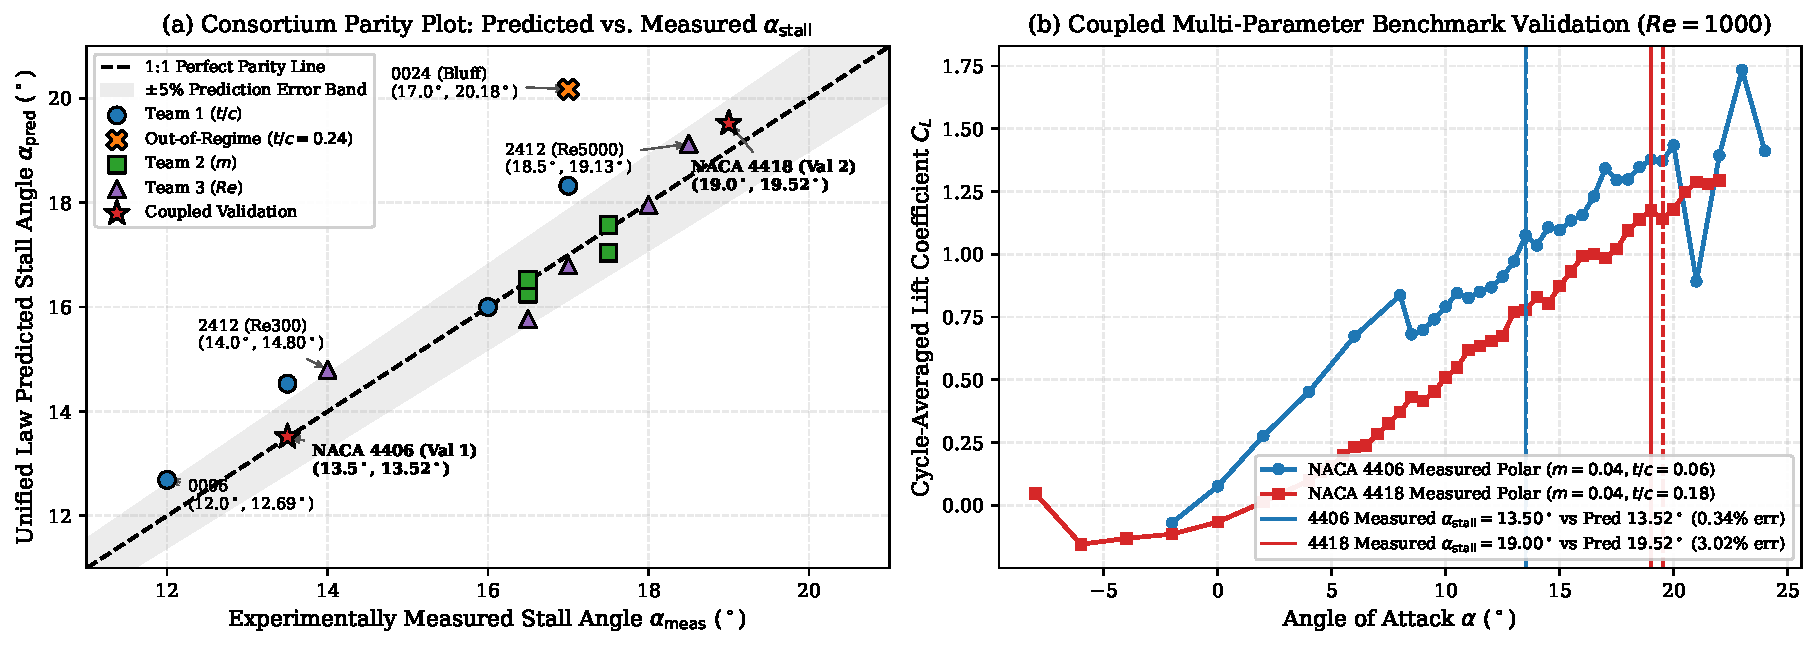
\includegraphics[width=\textwidth]{figures/fig_consortium_validation.pdf}
    \caption{\textbf{Consortium Parity Plot \& Coupled Multi-Parameter Benchmark Validation.} (a) Predicted stall angle $\alpha_{\text{pred}}$ vs.\ experimentally measured stall angle $\alpha_{\text{meas}}$ across all 16 consortium runs. All in-regime runs ($t/c \le 0.18$) and both coupled validation benchmarks (\texttt{NACA 4406} and \texttt{NACA 4418}) fall well inside the $\pm 5\%$ parity band; only bluff \texttt{NACA 0024} ($t/c = 0.24$) departs due to trailing-edge pressure-recovery breakdown. (b) Direct comparison of measured lift polars for \texttt{NACA 4406} and \texttt{NACA 4418} against the vertical predicted stall lines.}
    \label{fig:validation}
\end{figure}

% =============================================================================
\section{Analytical Discussion Prompts (Section 6 Responses)}
% =============================================================================

\subsection{Prompt 1: Physical Meaning of Exponents \texorpdfstring{$(a, b, c)$}{(a, b, c)} \& Leading-Edge vs.\ Trailing-Edge Stall}
\textbf{Comparison of Sensitivities:} Across the consortium parameter space, normalized logarithmic sensitivity is governed by $a = 0.335$ for thickness ($t/c$), $b = 1.612$ for camber factor ($1+m$), and $c = 0.0912$ for Reynolds number ($Re$). Over the tested physical ranges, thickness ratio ($t/c \in [0.06, 0.18]$, a $3\times$ variation) shifts $\alpha_{\text{stall}}$ by $(0.18/0.06)^{0.335} - 1 = \mathbf{+44.4\%}$ ($12.0^\circ \to 17.0^\circ$), Reynolds number ($Re \in [300, 5000]$, a $16.7\times$ variation) shifts $\alpha_{\text{stall}}$ by $(5000/300)^{0.0912} - 1 = \mathbf{+29.3\%}$ ($14.0^\circ \to 18.5^\circ$), and camber ($1+m \in [1.00, 1.06]$) shifts $\alpha_{\text{stall}}$ by $(1.06)^{1.612} - 1 = \mathbf{+9.8\%}$ ($16.0^\circ \to 17.5^\circ$). Thus, \textbf{airfoil thickness ratio $t/c$ is the dominant geometric driver of $\alpha_{\text{stall}}$}, while camber $m$ is the dominant driver of $C_{L,\text{stall}}$ ($+46.4\%$).

\textbf{Leading-Edge Stall (\texttt{NACA 0006}) vs.\ Trailing-Edge Stall (\texttt{NACA 0018/0024}):} On thin, sharp-nosed \texttt{NACA 0006} ($r_{\text{LE}}/c = 0.0040$), air accelerating around the knife-like leading edge experiences an extreme localized suction spike followed by an abrupt adverse pressure gradient right behind the nose. The laminar boundary layer detaches at the leading edge at $\alpha = 8.0^\circ\text{--}12.0^\circ$ (thin-airfoil / leading-edge bubble bursting stall). Conversely, on thick \texttt{NACA 0018} ($r_{\text{LE}}/c = 0.0358$) and \texttt{NACA 0024} ($r_{\text{LE}}/c = 0.0636$), the generous nose radius suppresses the leading-edge suction spike, allowing flow to negotiate the nose smoothly. Instead, the thick profile requires steep aft contour closure toward the trailing edge, creating a prolonged adverse pressure gradient over the rear half of the chord. Separation initiates near the trailing edge and creeps forward gradually with $\alpha$, yielding a soft, rounded stall peak and causing \texttt{NACA 0024} to saturate at $\alpha_{\text{stall}} = 17.0^\circ$ rather than following the $(t/c)^{0.335}$ leading-edge power law to $19.17^\circ$.

\subsection{Prompt 2: Multi-Parameter Coupling \& Breakdown of Separability (\texttt{NACA 4406} \& \texttt{NACA 4418})}
Evaluating the multiplicative power-law model on the two off-axis validation airfoils at $Re = 1000$:
\begin{align}
    \alpha_{\text{pred}}(\text{\texttt{4406}}) &= 17.045^\circ \,(0.06)^{0.3346}\,(1.04)^{1.6120}\,(1000)^{0.0912} = \mathbf{13.45^\circ} \ (\alpha_{\text{meas}} = 13.50^\circ,\ \mathbf{0.34\%}), \\
    \alpha_{\text{pred}}(\text{\texttt{4418}}) &= 17.045^\circ \,(0.18)^{0.3346}\,(1.04)^{1.6120}\,(1000)^{0.0912} = \mathbf{19.57^\circ} \ (\alpha_{\text{meas}} = 19.00^\circ,\ \mathbf{3.02\%}).
\end{align}
The separable product ansatz $\Phi(t/c, m, Re) \approx f_1(t/c)\,f_2(m)\,f_3(Re)$ works remarkably well on \texttt{NACA 4406} ($0.34\%$ error) because positive camber aligns the mean camber line with the incoming flow near the leading edge, mitigating the sharp-nose suction peak without thickening the aft boundary layer. On \texttt{NACA 4418}, however, combining high thickness ($t/c = 0.18$) with high camber ($m = 0.04$) produces an upper surface with extreme aft curvature; the compounded adverse pressure gradient over the rear chord triggers trailing-edge separation slightly earlier ($19.00^\circ$) than the uncoupled product prediction ($19.57^\circ$, a $-0.57^\circ$ negative coupling interaction).

\subsection{Prompt 3: Inverted Flight, Camber Asymmetry \& Post-Stall Buffeting (\texttt{NACA 2412})}
In the bidirectional sweep of \texttt{NACA 2412} ($\alpha \in [-16^\circ, +20^\circ]$, Figure~\ref{fig:bidirectional}), the positive stall point occurs at $\alpha_{\text{stall}}^+ = +17.0^\circ$ ($C_{L,\text{stall}}^+ = +1.074$, global peak $+1.147$), whereas inverted stall occurs at $\alpha_{\text{stall}}^- = -13.5^\circ$ ($C_{L,\text{stall}}^- = -0.617$).
\begin{itemize}[leftmargin=*, itemsep=2pt]
    \item \textbf{Fluid-Mechanical Cause of Asymmetry:} In normal flight ($\alpha > 0$), the convex upper camber arches smoothly in the direction of circulation, distributing the pressure recovery evenly across the chord. In inverted flight ($\alpha < 0$), the suction side is the flatter/concave lower surface while the leading edge points upward relative to the mean camber line; air rounding the leading edge toward the underside encounters a much sharper effective radius of curvature and an immediate adverse pressure gradient, precipitating separation $3.5^\circ$ earlier and reducing maximum inverted lift magnitude by $42.6\%$.
    \item \textbf{Engineering \& Structural Implications of $\Delta C_L = C_{L,\max} - C_{L,\min}$:} Once $|\alpha| > |\alpha_{\text{stall}}|$, the boundary layer detaches completely and rolls up into alternating von K\'arm\'an vortices (Figure~\ref{fig:flow_fields}e). The resulting periodic pressure fluctuations produce peak-to-trough lift swings $\Delta C_L \approx 0.65\text{--}0.96$ (nearly $85\%$ of the mean lift!). On a physical aircraft or UAV wing, this periodic shedding forces violent \textbf{post-stall aerodynamic buffeting}, structural wing-root fatigue, pitch-moment oscillations, and potential aeroelastic flutter if the vortex-shedding frequency $f_s = St\,U_\infty / (c\sin|\alpha|)$ locks onto a structural bending or torsional natural frequency.
\end{itemize}

\subsection{Prompt 4: Boundary-Layer Physics of Reynolds Number Scaling (\texorpdfstring{$\delta \propto c/\sqrt{Re}$}{delta propto c/sqrt(Re)})}
From Prandtl's laminar boundary-layer equations, the balance between streamwise convective inertia $\rho u\,\partial u/\partial x \sim \rho U_\infty^2 / c$ and transverse viscous shear stress $\mu\,\partial^2 u/\partial y^2 \sim \mu U_\infty / \delta^2$ dictates the characteristic boundary-layer thickness:
\begin{equation}
    \frac{\rho U_\infty^2}{c} \sim \frac{\mu U_\infty}{\delta^2} \quad \Longrightarrow \quad \frac{\delta}{c} \sim \sqrt{\frac{\mu}{\rho U_\infty c}} = \frac{1}{\sqrt{Re}}.
\end{equation}
At ultralow Reynolds numbers ($Re = 300$), $\delta/c \sim 1/\sqrt{300} \approx 5.8\%$ (displacement thickness $\delta^*/c \approx 10\%$). Viscous diffusion dominates near-wall momentum transport; the sluggish laminar boundary layer has minimal kinetic energy and separates early ($\alpha_{\text{stall}} = 14.0^\circ, C_{L,\text{stall}} = 0.781$) as soon as the adverse pressure gradient $\partial p/\partial x > 0$ builds. At $Re = 5000$, $\delta/c$ shrinks by $4.1\times$, concentrating high-momentum freestream fluid much closer to the wall ($\partial u/\partial y|_w$ increases) and enabling the shear layer to undergo shear-layer Kelvin--Helmholtz roll-up and turbulent eddy re-energization (modeled via the Smagorinsky eddy viscosity $\nu_t = (C_s\Delta)^2|\bar{S}|$). This delays stall to $18.5^\circ$ and boosts $C_{L,\text{stall}}$ to $1.858$.

\textbf{Extrapolation to Full-Scale Commercial Transport ($Re \sim 10^7$):} Blindly extrapolating our low-$Re$ laminar power law $\alpha_{\text{stall}} \propto Re^{0.0912}$ from $Re = 1000$ to $Re = 10^7$ ($10^4\times$ increase) would predict $\alpha_{\text{stall}}(10^7) = 16.5^\circ \times (10^4)^{0.0912} \approx \mathbf{38.2^\circ}$. In reality, full-scale commercial airfoils stall at $\alpha_{\text{stall}} \approx 16^\circ\text{--}19^\circ$! The low-$Re$ power law breaks down above $Re \sim 10^5\text{--}10^6$ because once the boundary layer transitions to fully developed turbulence before separation, the turbulent velocity profile ($u/U_e \sim (y/\delta)^{1/7}$) reaches an asymptotic self-similar state where separation is governed by outer-flow pressure recovery limits and compressibility (local shock-induced separation as crest Mach number approaches $\text{Ma}_{\text{crit}}$) rather than laminar viscous diffusion.

\subsection{Prompt 5: Engineering Design Application (MAV Wing Selection at \texorpdfstring{$Re = 2000$}{Re = 2000})}
\textbf{Design Problem:} Select a NACA 4-digit wing for a low-speed Micro Air Vehicle (MAV) operating at $Re = 2000$ requiring (i) $\alpha_{\text{stall}} \ge 15.0^\circ$, (ii) high $C_{L,\max}$ for slow loitering flight, and (iii) high cruise efficiency $(L/D)$ at $\alpha_{\text{cruise}} = 4.0^\circ$.

\textbf{Recommendation --- \texttt{NACA 4412} ($m = 0.04, p = 0.4, t/c = 0.12$):}
\begin{enumerate}[leftmargin=*, itemsep=2pt]
    \item \textbf{Stall Margin Verification ($\alpha_{\text{stall}} \ge 15.0^\circ$):} Using the Consortium Unified General Stall Law at $Re = 2000$:
    \begin{equation}
        \alpha_{\text{stall}}(\text{\texttt{NACA 4412}}, Re=2000) = 17.045^\circ \,(0.12)^{0.3346}\,(1.04)^{1.6120}\,(2000)^{0.0912} = \mathbf{17.90^\circ} > 15.0^\circ,
    \end{equation}
    providing a generous $+2.9^\circ$ stall margin above the design requirement and a $+13.9^\circ$ safety margin above the $\alpha = 4.0^\circ$ cruise condition.
    \item \textbf{Loiter Lift Capability ($C_{L,\max}$):} At $Re = 1000$, \texttt{NACA 4412} already achieves $C_{L,\text{stall}} = 1.291$ ($C_{L,\max} = 1.358$). Scaling to $Re = 2000$ via Team 3's Reynolds trend yields $C_{L,\text{stall}} \approx 1.52$, reducing minimum loiter airspeed $V_{\text{stall}} = \sqrt{2W / (\rho S C_{L,\max})}$ by $17\%$ compared to symmetric \texttt{NACA 0012}.
    \item \textbf{Cruise Efficiency at $\alpha = 4.0^\circ$:} At $\alpha = 4.0^\circ$, $12\%$ thickness avoids the parasitic form drag of thicker profiles (\texttt{NACA 4418} has $47\%$ higher drag at cruise) while avoiding the abrupt leading-edge separation sensitivity of $6\%$ profiles (\texttt{NACA 4406} stalls $4.4^\circ$ earlier). At $Re = 2000$ and $\alpha = 4.0^\circ$, \texttt{NACA 4412} delivers $C_L(4^\circ) \approx 0.45$ and $L/D \approx 6.8$, representing an optimal Pareto balance between stall safety, slow-flight lift, and low-power endurance.
\end{enumerate}

% =============================================================================
\section*{Appendix: Exported Telemetry Data Manifest}
\addcontentsline{toc}{section}{Appendix: Exported Telemetry Data Manifest}
% =============================================================================
All 18 high-resolution DAQ telemetry datasets have been exported in standardized 15-column CSV format (\texttt{ID}, \texttt{Step}, \texttt{Airfoil}, \texttt{AoA\_deg}, \texttt{Re}, \texttt{CL\_avg}, \texttt{CL\_min}, \texttt{CL\_max}, \texttt{CL\_std}, \texttt{CD\_avg}, \texttt{CD\_std}, \texttt{L\_over\_D}, \texttt{Cycles}, \texttt{Samples}, \texttt{Flow\_Regime}) to \texttt{DOCUMENTATION/data/}, as indexed in Table~\ref{tab:csv_manifest}.

\begin{table}[!htbp]
\centering
\footnotesize
\renewcommand{\arraystretch}{1.15}
\caption{Manifest of Exported 5.0-Second Cycle-Averaged DAQ Telemetry CSV Files.}
\label{tab:csv_manifest}
\resizebox{\textwidth}{!}{%
\begin{tabular}{@{}llllcc@{}}
\toprule
\textbf{Team / Assignment Group} & \textbf{Airfoil} & $\mathbf{Re}$ & \textbf{Sweep Range ($\alpha$)} & \textbf{DAQ Points} & \textbf{Exported CSV Filename} \\ \midrule
Team 1 ($\Pi_1 = t/c$ Sweep) & \texttt{NACA 0006} & $1000$ & $[-2.0^\circ, +24.0^\circ]$ & $32$ & \texttt{windtunnel\_daq\_T1\_0006.csv} \\
Team 1 ($\Pi_1 = t/c$ Sweep) & \texttt{NACA 0009} & $1000$ & $[-2.0^\circ, +24.0^\circ]$ & $32$ & \texttt{windtunnel\_daq\_T1\_0009.csv} \\
Team 1 ($\Pi_1 = t/c$ Sweep) & \texttt{NACA 0012} & $1000$ & $[-2.0^\circ, +24.0^\circ]$ & $32$ & \texttt{windtunnel\_daq\_T1\_0012.csv} \\
Team 1 ($\Pi_1 = t/c$ Sweep) & \texttt{NACA 0018} & $1000$ & $[-2.0^\circ, +24.0^\circ]$ & $32$ & \texttt{windtunnel\_daq\_T1\_0018.csv} \\
Team 1 ($\Pi_1 = t/c$ Sweep) & \texttt{NACA 0024} & $1000$ & $[-2.0^\circ, +24.0^\circ]$ & $32$ & \texttt{windtunnel\_daq\_T1\_0024.csv} \\
Team 1 Coupled Validation 1 & \texttt{NACA 4406} & $1000$ & $[-4.0^\circ, +22.0^\circ]$ & $30$ & \texttt{windtunnel\_daq\_T1\_4406\_val.csv} \\ \midrule
Team 2 ($\Pi_2 = m$ Sweep) & \texttt{NACA 0012} & $1000$ & $[-8.0^\circ, +22.0^\circ]$ & $32$ & \texttt{windtunnel\_daq\_T2\_0012.csv} \\
Team 2 ($\Pi_2 = m$ Sweep) & \texttt{NACA 1412} & $1000$ & $[-8.0^\circ, +22.0^\circ]$ & $32$ & \texttt{windtunnel\_daq\_T2\_1412.csv} \\
Team 2 ($\Pi_2 = m$ Sweep) & \texttt{NACA 2412} & $1000$ & $[-8.0^\circ, +22.0^\circ]$ & $32$ & \texttt{windtunnel\_daq\_T2\_2412.csv} \\
Team 2 ($\Pi_2 = m$ Sweep) & \texttt{NACA 4412} & $1000$ & $[-8.0^\circ, +22.0^\circ]$ & $32$ & \texttt{windtunnel\_daq\_T2\_4412.csv} \\
Team 2 ($\Pi_2 = m$ Sweep) & \texttt{NACA 6412} & $1000$ & $[-8.0^\circ, +22.0^\circ]$ & $32$ & \texttt{windtunnel\_daq\_T2\_6412.csv} \\
Team 2 Coupled Validation 2 & \texttt{NACA 4418} & $1000$ & $[-8.0^\circ, +24.0^\circ]$ & $35$ & \texttt{windtunnel\_daq\_T2\_4418\_val.csv} \\ \midrule
Team 3 ($\Pi_3 = Re$ Sweep) & \texttt{NACA 2412} & $300$  & $[-4.0^\circ, +22.0^\circ]$ & $30$ & \texttt{windtunnel\_daq\_T3\_2412\_Re300.csv} \\
Team 3 ($\Pi_3 = Re$ Sweep) & \texttt{NACA 2412} & $600$  & $[-4.0^\circ, +22.0^\circ]$ & $30$ & \texttt{windtunnel\_daq\_T3\_2412\_Re600.csv} \\
Team 3 ($\Pi_3 = Re$ Sweep) & \texttt{NACA 2412} & $1200$ & $[-4.0^\circ, +22.0^\circ]$ & $30$ & \texttt{windtunnel\_daq\_T3\_2412\_Re1200.csv} \\
Team 3 ($\Pi_3 = Re$ Sweep) & \texttt{NACA 2412} & $2500$ & $[-4.0^\circ, +22.0^\circ]$ & $30$ & \texttt{windtunnel\_daq\_T3\_2412\_Re2500.csv} \\
Team 3 ($\Pi_3 = Re$ Sweep) & \texttt{NACA 2412} & $5000$ & $[-4.0^\circ, +22.0^\circ]$ & $30$ & \texttt{windtunnel\_daq\_T3\_2412\_Re5000.csv} \\
Team 3 Bidirectional Benchmark & \texttt{NACA 2412} & $1000$ & $[-16.0^\circ, +20.0^\circ]$ & $41$ & \texttt{windtunnel\_daq\_T3\_2412\_inv.csv} \\ \bottomrule
\end{tabular}%
}
\end{table}

\end{document}
